\chapter{周波数解析}
\section{\kadaiba}\label{sec:\kadaiba}
\purpose
\matlab を用いて周波数解析を行う.我々が普段見る「波形」は時間軸を横,振幅を縦にしたグラフである.
このグラフからわかるのは時刻に対しての振幅だ.ただし波形の分析はそれだけでは不十分である.
波形というのはフーリエ級数展開の理論により,いかなる波形も\eqref{equ:フーリエ級数展開}の\(N=\infty\)で表せる.
波形に対してフーリエ変換を行うと「周波数に対する振幅」を得ることができる.矩形波\eqref{equ:矩形波}の振幅と周波数をグラフに描画したものを振幅スペクトルと呼ぶ.(\ref{fig:周波数解析})\par
今回の実験では,純音と矩形波に対して演算を施し周波数解析を行う.周波数に対しての振幅をグラフに描画し,どの周波数成分が多いか確認する.
\begin{figure}[H]
    \centering
    \begin{minipage}{.4\textwidth}
    \renewcommand{\arraystretch}{1.5}
    \centering
    \begin{tabular}[c]{r|cc}
        \multicolumn{1}{c}{正弦波}   & 振幅                                                            & 周波数                                                             \\
        \hline
        \(2\sin(t)\)              & \tikz[remember picture,baseline=(A.base)]{\node(A){\(2\)}}    & \tikz[remember picture,baseline=(D.base)]{\node(D){\(1/2\pi\)}} \\
        \(-\sin (2t)\)            & \(-1\)                                                        & \(1/\pi\)                                                       \\
        \(\frac{2}{3}\sin (3t)\)  & \(2/3\)                                                       & \(3/2\pi\)                                                      \\
        \(-\frac{1}{2}\sin (4t)\) & \tikz[remember picture,baseline=(C.base)]{\node(C){\(-1/2\)}} & \tikz[remember picture,baseline=(B.base)]{\node(B){\(2/\pi\)}}  \\
        \multicolumn{3}{c}{{\LARGE\vdots}}
    \end{tabular}
    \begin{tikzpicture}[remember picture,overlay]
        \node[inner sep=0.1mm,fit={(A)(B)(C)(D)},draw,rounded corners,draw=blue](warp){};
    \end{tikzpicture}
    \begin{align*}
        f(t) & =\sum_{k=1}^{N}\frac{1}{2k-1}\sin\big(2\pi(2s-1)ft\big)\tag*{(\ref{equ:矩形波})}
    \end{align*}
\end{minipage}
\begin{minipage}{.4\textwidth}
    \centering
    \begin{tikzpicture}[remember picture]
        \node[left] at(0,0){O};
        \draw[very thick,-Stealth](0,0)--(5,0)node[midway,fill=white]{\scriptsize 周波数};
        \draw[very thick,-Stealth](0,-1.6)--(0,4.1)node[left]at($(0,0)!0.5!(0,4.1)$){\scriptsize \rotatebox{90}{振幅}};
        \foreach \u \v in {0.4/3,0.8/-1.5,1.2/1,1.6/-0.75}
        \draw[thick,blue](\u,0)--(\u,\v);
        \foreach \u \v \z in {0.4/{\(1/2\pi\)}/below,0.8/{\(1/\pi\)}/above,1.2/{\(3/2\pi\)}/below,1.6/{\(2/\pi\)}/above}
        \node[\z] at(\u,0){\tiny\v};
        \coordinate (O) at (0,0);
        \foreach \u \v \z \w in {0.4/3/a/{\(2\)},0.8/-1.5/b/{\(-1\)},1.2/1/c/{\(2/3\)},1.6/-0.75/d/{\(-1/2\)}} {
        \coordinate (\z) at (\u,\v);
        \draw[dotted,thin](\z)--(O |- \z)node[left]{\tiny\w};
        }
    \end{tikzpicture}
    \begin{tikzpicture}[remember picture,overlay]
        \draw[-latex,very thick,dashed]($(warp.south east)!0.5!(warp.north east)$)--($(O)+(-0.5cm,0)$);
    \end{tikzpicture}
\end{minipage}
    \caption{周波数解析}
    \label{fig:周波数解析}
\end{figure}
\method
\paragraph{高速フーリエ変換の実装}
\matlab ではデータ列\texttt{y}に対して高速フーリエ変換をする関数\texttt{fft(y)}がある.
ただし,\texttt{fft}関数の仕様上いくつかの注意が必要である.データ列\texttt{y}に対して振幅スペクトルを取得する手順は以下の通りである.
\begin{enumerate}
    \item 高速フーリエ変換を行う.(\texttt{y\_fft=fft(y)})\\
          \texttt{fft}関数は出力として,サンプリング周波数\texttt{Fs}に対して,\(\big[\textrm{\texttt{-Fs/2}},\textrm{\texttt{Fs/2}}\big]\)範囲の周波数に対する振幅のデータを得る.
    \item 出力データ列\texttt{fft(y)}のデータを整列させる.(\texttt{y\_fft=fftshift(y\_fft)})\\
          \texttt{fft}関数の出力は,正のデータ・負のデータ(左右)が入れ替わった状態で出力される.
    \item これまでの過程で出力されるデータは複素数データである.絶対値を取るために\texttt{abs}関数を用いる.
    \item グラフとして描画するために,周波数軸を作成する.
\end{enumerate}
\begin{figure}[h]
    \centering
    \begin{minipage}[b]{.48\textwidth}
        \centering
        \begin{tikzpicture}
    \fill[fill=blue,opacity=0.1]($(.9\textwidth,0.5)!0.5!(0,0.5)$)rectangle(.9\textwidth,0);
    \fill[fill=red,opacity=0.1](0,0)rectangle($(.9\textwidth,0.5)!0.5!(0,0.5)$);
    \draw[thick](0,0)--(0.9\textwidth,0)--(0.9\textwidth,0.5)--(0,0.5)--cycle;
    \node[below] at (0,0)(a){\tiny\texttt{1}};
    \node[above] at (0,0.5){\tiny\texttt{0}};
    \node[above left] at ($(.9\textwidth,0.5)!0.5!(0,0.5)$){\tiny\texttt{Fs/2}};
    \node[above right] at ($(.9\textwidth,0.5)!0.5!(0,0.5)$){\tiny\texttt{-Fs/2}};
    \node[above] at (.9\textwidth,0.5){\tiny\texttt{-1/Fs}};
    \node[below] at (0.9\textwidth,0)(b){\tiny\texttt{Fs}};
    \draw[latex-latex](a)--(b)node[midway,below]{\tiny\texttt{index}};
    \coordinate (C) at ($(0.9\textwidth,0)!0.5!(0,0)$);
    \draw[thick](C)--($(C)+(0,1.5mm)$);
    \coordinate (c) at ($(0.9\textwidth,0.5)!0.5!(0,0.5)$);
    \draw[thick](c)--($(c)+(0,-1.5mm)$);
    \node at($(C)!0.5!(0,5mm)$){\tiny 正のデータ};
    \node at($(c)!0.5!(0.9\textwidth,0mm)$){\tiny 負のデータ};
\end{tikzpicture}
        \caption{\texttt{fft}直後の出力データ}
        \label{fig:fft直後のデータ}
    \end{minipage}
    \begin{minipage}[b]{.48\textwidth}
        \centering
        \begin{tikzpicture}
    \fill[fill=red,opacity=0.1]($(.9\textwidth,0.5)!0.5!(0,0.5)$)rectangle(.9\textwidth,0);
    \fill[fill=blue,opacity=0.1](0,0)rectangle($(.9\textwidth,0.5)!0.5!(0,0.5)$);
    \draw[thick](0,0)--(0.9\textwidth,0)--(0.9\textwidth,0.5)--(0,0.5)--cycle;
    \node[below] at (0,0)(a){\tiny\texttt{1}};
    \node[above] at (0,0.5){\tiny\texttt{-Fs/2}};
    \node[above left] at ($(.9\textwidth,0.5)!0.5!(0,0.5)$){\tiny\texttt{-1/Fs}};
    \node[above right] at ($(.9\textwidth,0.5)!0.5!(0,0.5)$){\tiny\texttt{0}};
    \node[above] at (.9\textwidth,0.5){\tiny\texttt{Fs/2}};
    \node[below] at (0.9\textwidth,0)(b){\tiny\texttt{Fs}};
    \draw[latex-latex](a)--(b)node[midway,below]{\tiny\texttt{index}};
    \coordinate (C) at ($(0.9\textwidth,0)!0.5!(0,0)$);
    \draw[thick](C)--($(C)+(0,1.5mm)$);
    \coordinate (c) at ($(0.9\textwidth,0.5)!0.5!(0,0.5)$);
    \draw[thick](c)--($(c)+(0,-1.5mm)$);
    \node at($(C)!0.5!(0,5mm)$){\tiny 負のデータ};
    \node at($(c)!0.5!(0.9\textwidth,0mm)$){\tiny 正のデータ};
\end{tikzpicture}
        \caption{\texttt{fftshift}後の出力データ}
        \label{fig:fftshift後のデータ}
    \end{minipage}
    \begin{minipage}[b]{.48\textwidth}
        \centering
        \begin{tikzpicture}
    \node(fig){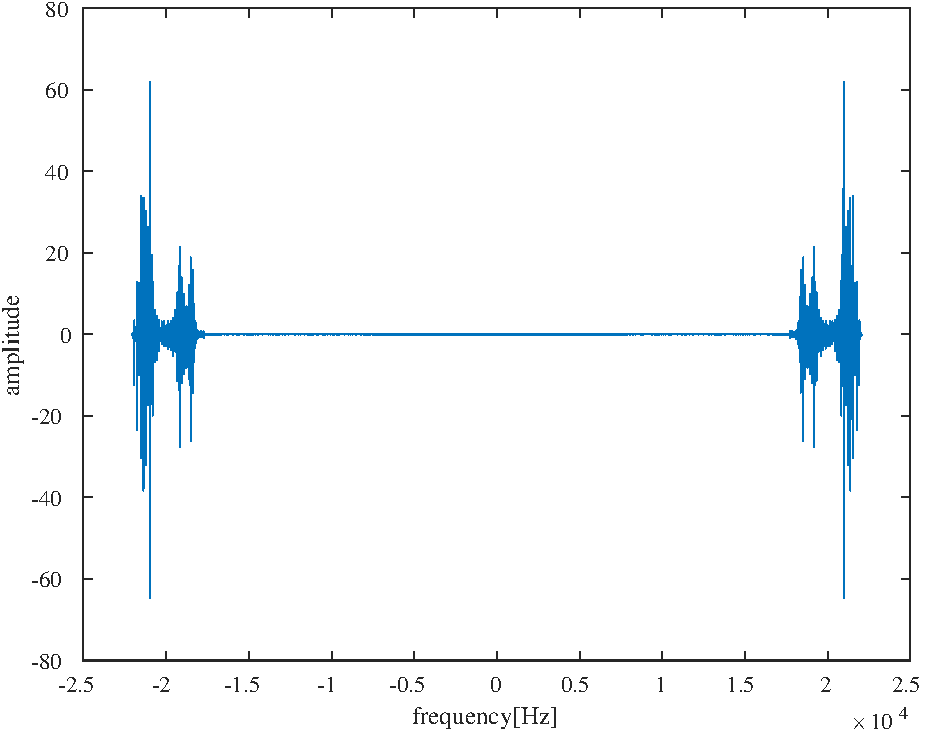
\includegraphics[keepaspectratio,width=.9\textwidth]{Figures/fft_fft.pdf}};
    \coordinate (figsouth) at (fig.south);
    \coordinate (figscenter) at ($(figsouth)+(2.75mm,7.1mm)$);
    \coordinate (figncenter) at ($(figscenter)+(0,5.48cm)$);
    \coordinate (figsleft) at ($(figscenter)+(-3.47cm,0)$);
    \coordinate (figsright) at ($(figscenter)+(3.47cm,0)$);
    \fill[fill=red,opacity=0.1](figsleft)--(figsleft |- figncenter)--(figncenter)--(figscenter)--cycle;
    \fill[fill=blue,opacity=0.1](figsright)--(figsright |- figncenter)--(figncenter)--(figscenter)--cycle;
    \coordinate (L) at($(figncenter)!0.5!(figsleft)+(0,1cm)$);
    \coordinate (R) at($(figncenter)!0.5!(figsright)+(0,1cm)$);
    \draw[very thick,dashed,latex-latex](L)to[bend left=40](R);
\end{tikzpicture}
        \caption{\texttt{fft}直後の出力データ(グラフ)}
        \label{fig:fft直後のデータ(グラフ)}
    \end{minipage}
    \begin{minipage}[b]{.48\textwidth}
        \centering
        \begin{tikzpicture}
    \node(fig){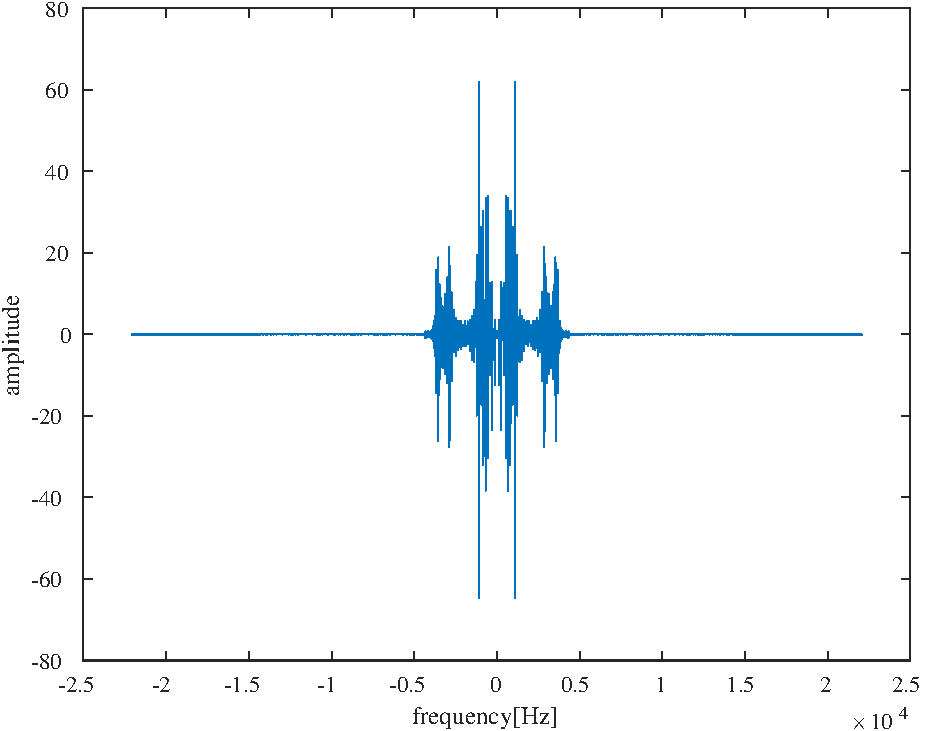
\includegraphics[keepaspectratio,width=.9\textwidth]{Figures/fft_fftshift.pdf}};
    \coordinate (figsouth) at (fig.south);
    \coordinate (figscenter) at ($(figsouth)+(2.75mm,7.1mm)$);
    \coordinate (figncenter) at ($(figscenter)+(0,5.48cm)$);
    \coordinate (figsleft) at ($(figscenter)+(-3.47cm,0)$);
    \coordinate (figsright) at ($(figscenter)+(3.47cm,0)$);
    \fill[fill=blue,opacity=0.1](figsleft)--(figsleft |- figncenter)--(figncenter)--(figscenter)--cycle;
    \fill[fill=red,opacity=0.1](figsright)--(figsright |- figncenter)--(figncenter)--(figscenter)--cycle;
\end{tikzpicture}
        \caption{\texttt{fftshift}後の出力データ(グラフ)}
        \label{fig:fftshift後のデータ(グラフ)}
    \end{minipage}
    \begin{minipage}{.48\textwidth}
        \centering
        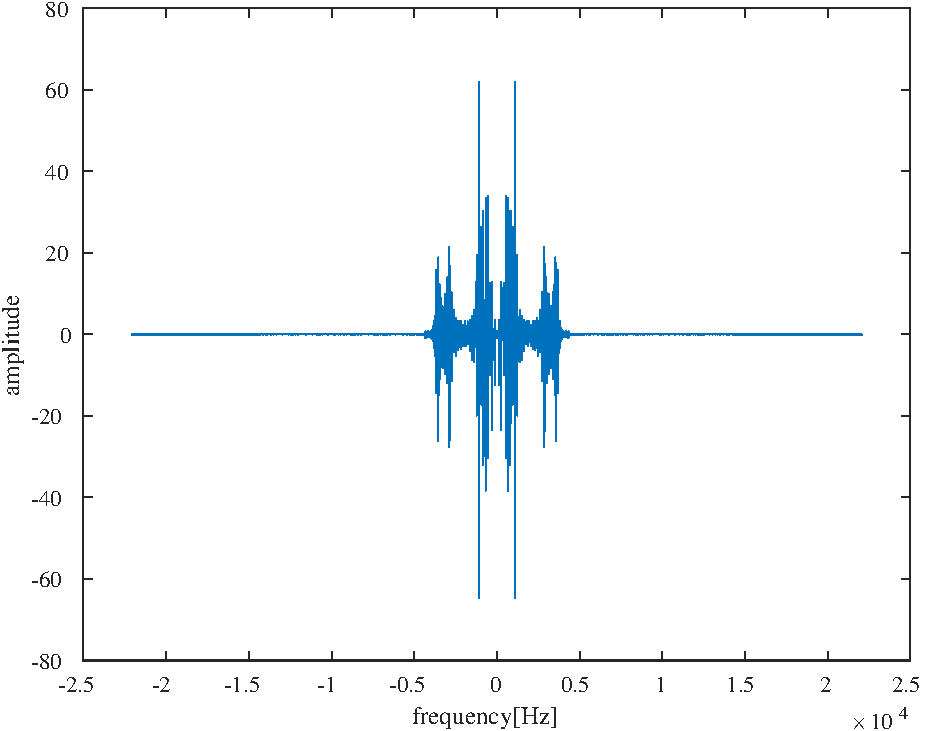
\includegraphics[keepaspectratio,width=.9\textwidth]{Figures/fft_fftshift.pdf}
    \end{minipage}
    \begin{minipage}{.48\textwidth}
        \centering
        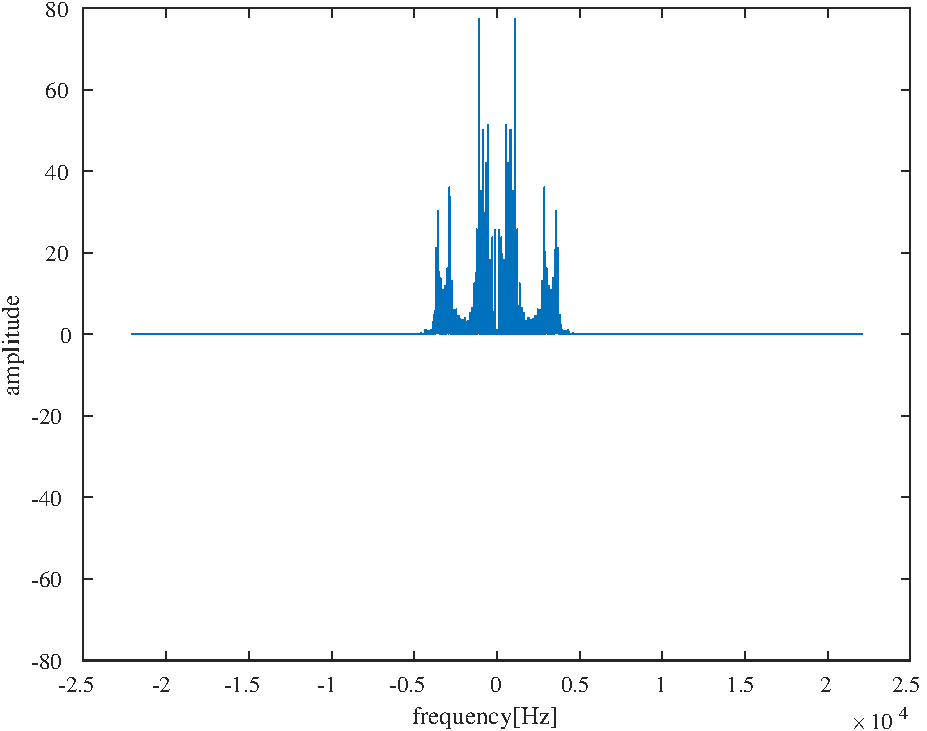
\includegraphics[keepaspectratio,width=.9\textwidth]{Figures/fft_abs.pdf}
    \end{minipage}
\end{figure}
\section{\kadaibb}\label{sec:\kadaibb}